%
%  exercise-1.tex
%  artificial intelligence
%
%  Created by Illya Starikov on 01/17/18.
%  Copyright 2018. Illya Starikov. All rights reserved.
%

\RequirePackage[l2tabu, orthodox]{nag}
\documentclass[12pt]{scrartcl}

\newcommand{\exercisenumber}{4}
\newcommand{\duedate}{July 20\textsuperscript{th}, 2018}
\usepackage{amssymb,amsmath,verbatim,graphicx,microtype,upquote,units,booktabs,akkwidepage}

\newcommand{\chapterNumber}[1]{
    \setcounter{section}{#1}
    \addtocounter{section}{-1}
}
\usepackage[shortlabels]{enumerate}
\usepackage{multicol}

\begin{document}
\maketitle

\section{Support Vector Machine}
\begin{enumerate}[a)]

    \item Our equations would be as follows:

    \begin{align*}
        \alpha_1\,\varphi\left(s_1\right) \cdot \varphi\left(s_1\right) + \alpha_2\,\varphi\left(s_2\right) \cdot \varphi\left(s_1\right) &= 1 \\
        \alpha_1\,\varphi\left(s_1\right) \cdot \varphi\left(s_2\right) + \alpha_2\,\varphi\left(s_2\right) \cdot \varphi\left(s_2\right) &= -1 \\
    \end{align*}

    \item Assuming $\varphi$ to be the identity operator, we get as follows:

        % (2, 1, 1) = s_1
        % (4, 2, 1) = s_2

        \begin{align*}
            6\, \alpha_1 + 11\, \alpha_2 &= 1 \\
            11\, \alpha_1 + 21\, \alpha_2 &= -1 \\
        \end{align*}

        From this, we get as follows:

        \begin{equation*}
            \alpha_1 = \nicefrac{32}{5} \qquad \alpha_2 = -\nicefrac{17}{5}
        \end{equation*}

    \item Our discriminating hyperplane would be as follows:

        \begin{equation*}
            w' = <-\nicefrac{4}{5}, -\nicefrac{2}{5}, 3>
        \end{equation*}

        Therefore, the plane equation would be as follows:

        \begin{equation*}
            -\nicefrac{4}{5}\,x -\nicefrac{2}{5}\,y + 3 = 0
        \end{equation*}
\end{enumerate}

\section{K2 Bayesian Network}
For our $\alpha$ values, we get the following:

\begin{align*}
    \alpha_{411} = 1 &\quad(\textit{\# cases with $x_1 = 0$, $x_2 = N$, $x_4 = H$}) \\
    \alpha_{412} = 2 &\quad(\textit{\# cases with $x_1 = 0$, $x_2 = N$, $x_4 = L$}) \\
    \alpha_{413} = 1 &\quad(\textit{\# cases with $x_1 = 0$, $x_2 = N$, $x_4 = M$}) \\
    \alpha_{421} = 0 &\quad(\textit{\# cases with $x_1 = 0$, $x_2 = Y$, $x_4 = H$}) \\
    \alpha_{422} = 3 &\quad(\textit{\# cases with $x_1 = 0$, $x_2 = Y$, $x_4 = L$}) \\
    \alpha_{423} = 1 &\quad(\textit{\# cases with $x_1 = 0$, $x_2 = Y$, $x_4 = M$}) \\
    \alpha_{431} = 1 &\quad(\textit{\# cases with $x_1 = 1$, $x_2 = N$, $x_4 = H$}) \\
    \alpha_{432} = 3 &\quad(\textit{\# cases with $x_1 = 1$, $x_2 = N$, $x_4 = L$}) \\
    \alpha_{433} = 1 &\quad(\textit{\# cases with $x_1 = 1$, $x_2 = N$, $x_4 = M$}) \\
    \alpha_{441} = 0 &\quad(\textit{\# cases with $x_1 = 1$, $x_2 = Y$, $x_4 = H$}) \\
    \alpha_{442} = 2 &\quad(\textit{\# cases with $x_1 = 1$, $x_2 = Y$, $x_4 = L$}) \\
    \alpha_{443} = 1 &\quad(\textit{\# cases with $x_1 = 1$, $x_2 = Y$, $x_4 = M$}) \\
\end{align*}

For our $N$ values, we get the following:

\begin{align*}
    N_{41} = \alpha_{411} + \alpha_{412} + \alpha_{413} &= 1 + 2 + 1 = 4\\
    N_{42} = \alpha_{421} + \alpha_{422} + \alpha_{423} &= 0 + 3 + 1 = 4\\
    N_{43} = \alpha_{431} + \alpha_{432} + \alpha_{433} &= 1 + 3 + 1 = 5\\
    N_{44} = \alpha_{441} + \alpha_{442} + \alpha_{443} &= 0 + 2 + 1 = 3\\
\end{align*}

\section{Weka Output}
\begin{figure}[H]
    \centering
    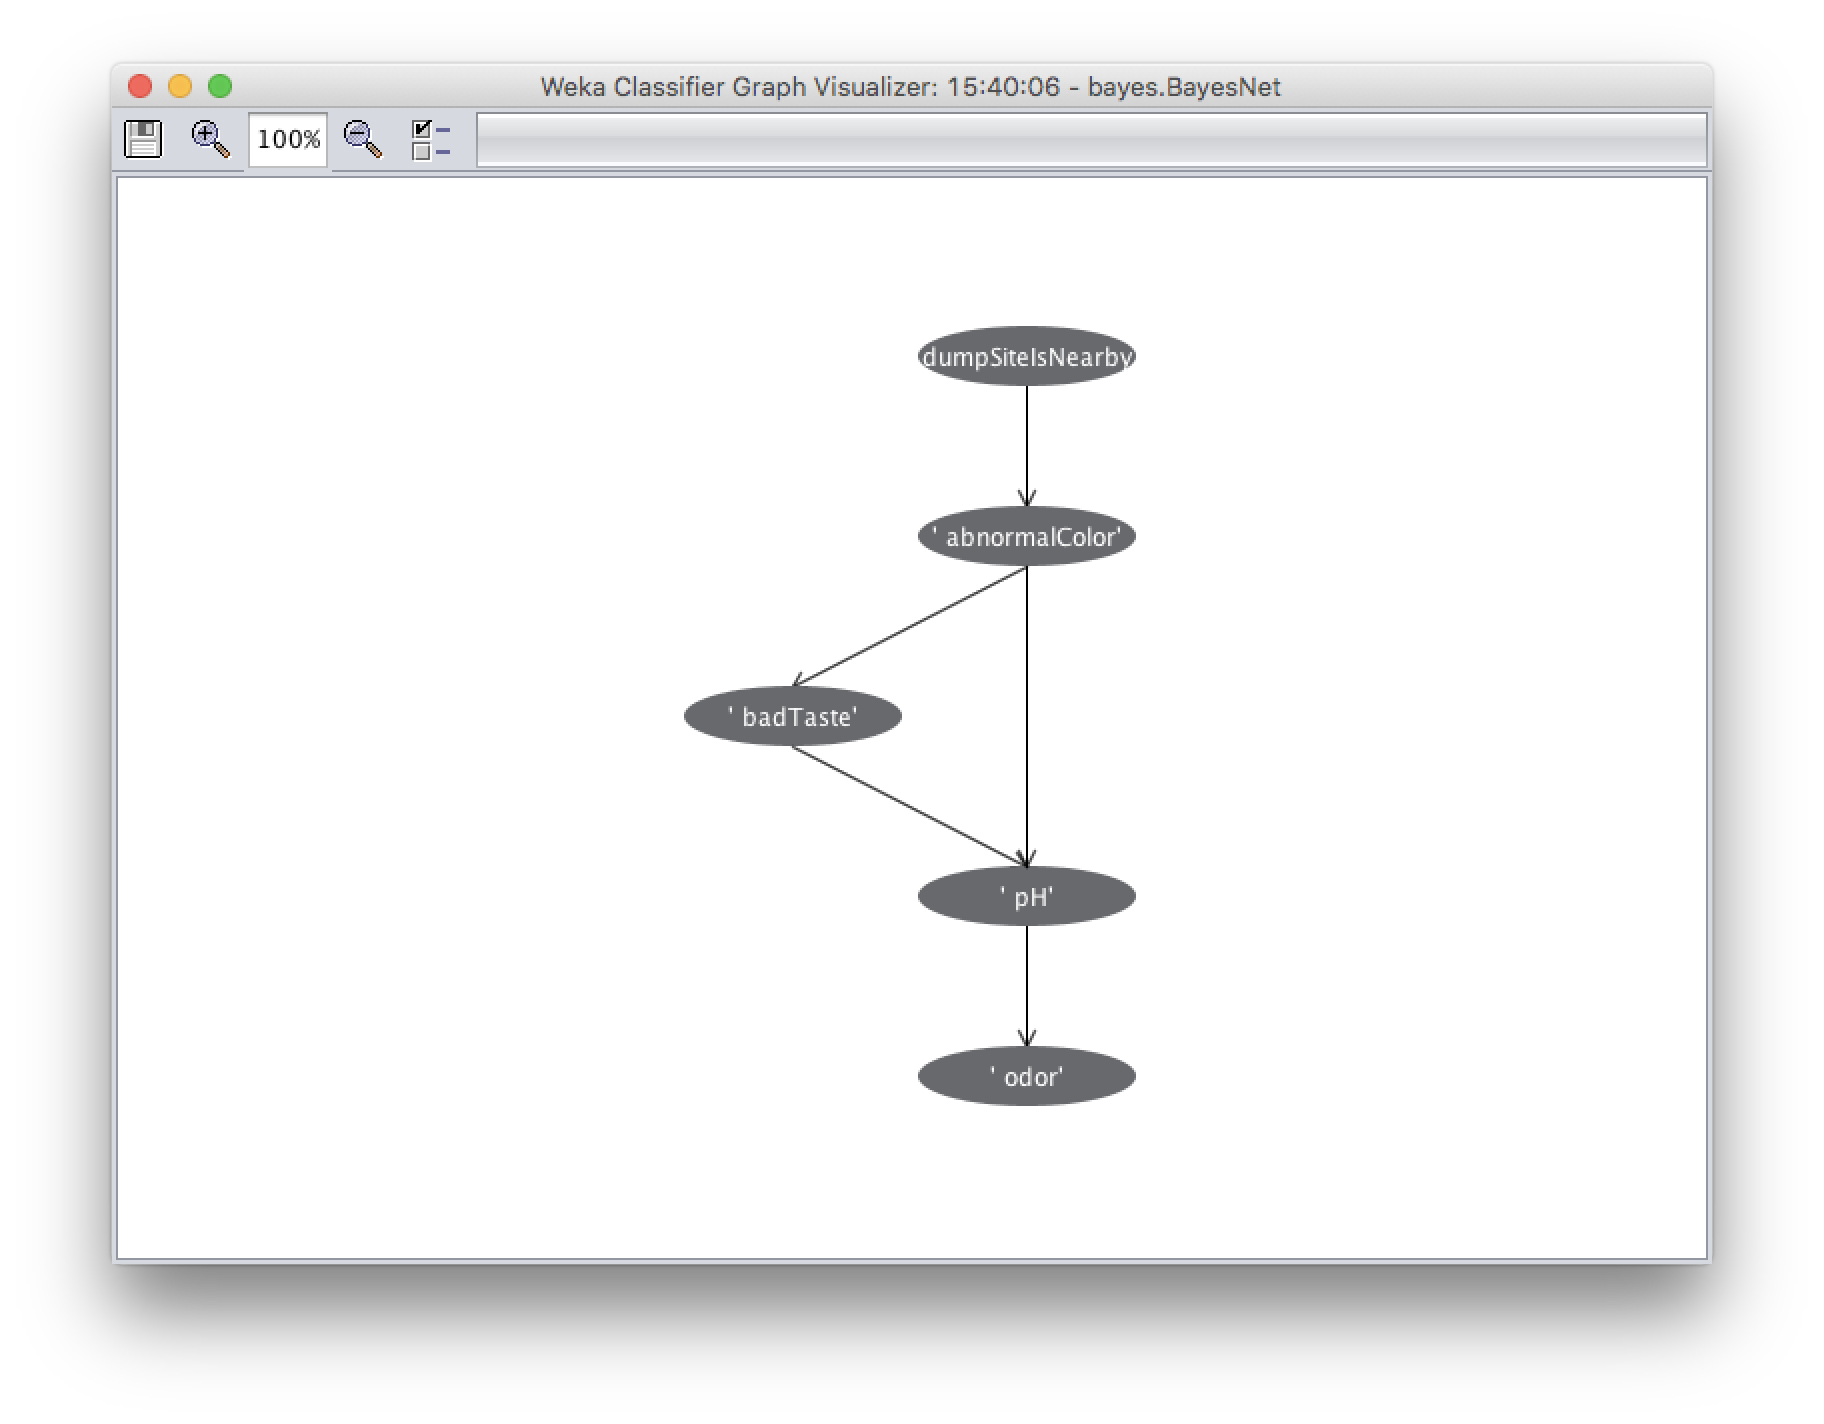
\includegraphics[width=0.8\linewidth]{assets/example-3}
\end{figure}

For the Niave vs Regular Bayesian Network, the results are similar. With the same confusion matrix, they both correct and correctly classify the same number of instances (and the same instances).

\section{K2}
From the graph, we can first determine that $x_5$ is not dependent on $x_1, x_2, x_3$ or $x_4$. However, $x_3$ and $x_4$ depend on $x_2$ (from the arrows being directed from $x_2$ to $x_3$ and $x_4$). Likewise, $x_2$ depends on $x_1$.


\end{document}
